\documentclass[a4paper,12pt]{article}

%% Language and font encodings
\usepackage[english, russian]{babel}
\usepackage[utf8x]{inputenc}
\usepackage{blindtext}
\usepackage[T1]{fontenc}
\usepackage[T2A]{fontenc}
\usepackage[a4paper,top=1.5 cm,bottom=2cm,left=3cm,right=3cm,marginparwidth=1.75cm]{geometry}
%% Useful packages
\usepackage{amsmath, amssymb}
\usepackage{wrapfig}
\usepackage{graphicx}
\usepackage[usenames]{color}
\usepackage[T1]{fontenc}
\usepackage{tikz}
\usetikzlibrary{arrows}
\usetikzlibrary{decorations.pathreplacing}
\usepackage[T2A]{fontenc}
\usepackage{color}
\usepackage{circuitikz} 
\usetikzlibrary{circuits}
\usetikzlibrary{circuits.ee}
\usetikzlibrary{circuits.ee.IEC}
\usetikzlibrary{circuits.logic.IEC}
\graphicspath{{pic/}}
\definecolor{water} {rgb} {0.667, 0.855, 1}
\usepackage{pgfplots}
\usepackage{pgfplotstable}

\title{ИЗУЧЕНИЕ ДИФРАКЦИИ СВЕТА}
\date{Работа 4.3.1}
\author{Ляликова Ирина, Б05-911}
\begin{document}
	
	\vspace{0.5 cm}
	\maketitle
	\vspace{0.5 cm}
	
	\textbf{Цель работы:} Исследовать дифракцию Френеля на узкой щели, на краю экрана, на тонкой нити; исследовать дифракцию Фраунгофера на щели и проследить, как влияют изменение ширины щели и её смещение на характер дифракционной картины; исследовать картину дифракции на двух щелях и оценить влияние размеров источника на чёткость картины; исследовать влияние дифракции на разрешающую способность оптических инструментов.
	
	\textbf{В работе используются:} оптическая скамья, ртутная лампа, монохроматор, щели с регулируемой шириной, рамка с вертикальной нитью, двойная щель, микроскоп на поперечных салазках с микрометрическим винтом, зрительная труба.
	
	\section*{Теоретическое введение и установка}
	\subsection*{А. Дифракция Френеля}
	
	Схема установки для наблюдения дифракции Френеля представлена на рис. 1. Световые лучи освещают щель~$S_2$ и испытывают на ней дифракцию. Дифракционная картина рассматривается с помощью микроскопа~М, сфокусированного на некоторую плоскость наблюдения~П.
		\begin{figure}[h]
		\begin{center}
			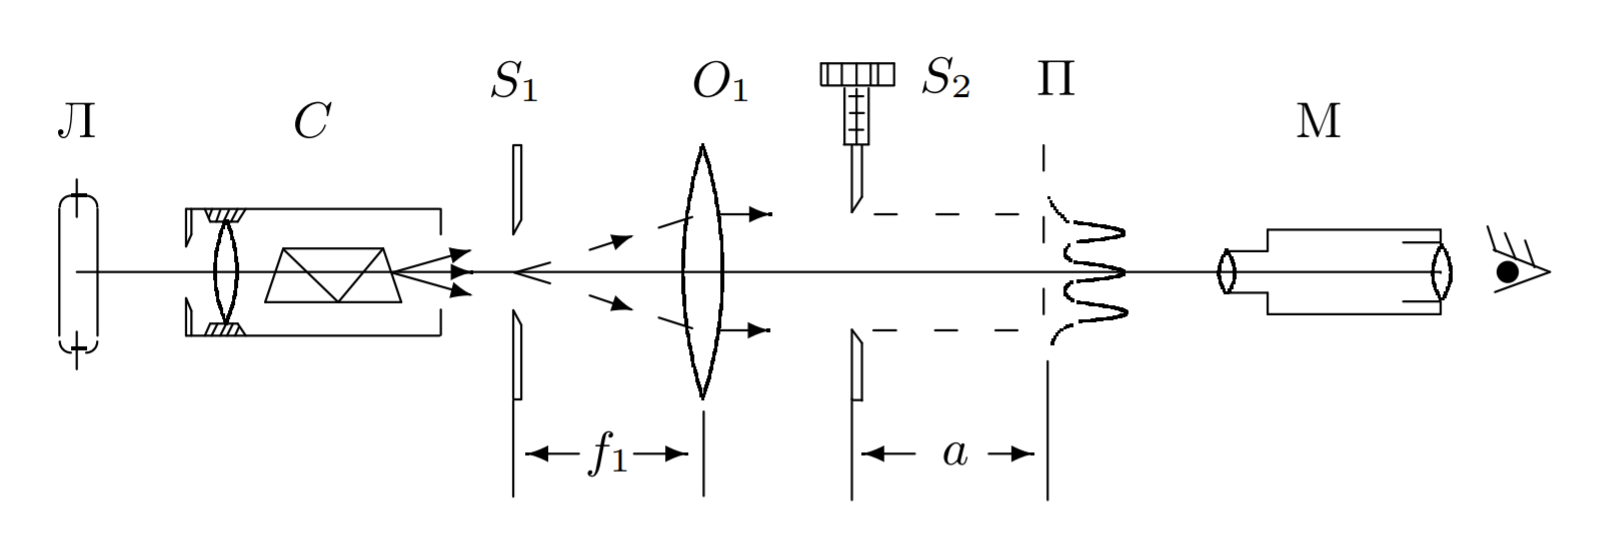
\includegraphics[width = 0.7\textwidth]{431-1.png}
			\caption{Схема установки для наблюдения дифракции Френеля}
		\end{center}
	\end{figure}
	
	Щель~$S_2$ освещается параллельным пучком монохроматического света с помощью коллиматора, образованного объективом~$O_1$ и щелью~$S_1$, находящейся в его фокусе. На щель~$S_1$ сфокусировано изображение спектральной линии, выделенной из спектра ртутной лампы~Л при помощи простого монохроматора~C.
	
	
	Распределение интенсивности света в плоскости наблюдения~П проще всего рассчитывать с помощью зон Френеля (для щели их иногда называют зонами Шустера). При освещении щели~$S_2$ параллельным пучком лучей (плоская волна) зоны Френеля представляют собой полоски, параллельные краям щели (рис. 2). Результирующая амплитуда в точке наблюдения определяется суперпозицией колебаний от тех зон Френеля, которые не перекрыты створками щели. Графическое определение результирующей амплитуды производится с помощью векторной диаграммы --- спирали Корню. Суммарная ширина $m$ зон Френеля $z_m$ определяется соотношением
	\begin{equation}
	z_m=\sqrt{am\lambda},
	\end{equation}
	где $a$ --- расстояние от щели до плоскости наблюдения (рис. 1), а $\lambda$ --- длина волны.
	
	Вид наблюдаемой дифракционной картины определяется числом Френеля $\Phi$: квадрат числа Френеля
	\begin{equation*}
	\Phi^2 = \dfrac{D}{\sqrt{a\lambda}}.
	\end{equation*}
	Дифракционная картина отсутствует, когда плоскость наблюдения~П совпадает с плоскостью щели: при $\Phi \rightarrow \infty$ мы имеем дело с геометрической оптикой. При небольшом удалении от щели, когда число Френеля $\Phi \gg 1$ (на щели укладывается огромное число зон), дифракционная картина наблюдается только в узкой области на границе света и тени у краёв экрана.
	
	При последующем небольшом удалении от щели (или изменении ширины щели $S_2$) эти две группы дифракционных полос перемещаются практически независимо друг от друга. При дальнейшем увеличении расстояния (или уменьшении ширины щели~$S_2$) обе системы дифракционных полос постепенно сближаются и, наконец, при $\Phi \gtrsim 1$ накладываются друг на друга. Распределение интенсивности в плоскости наблюдения в этом случае определяется числом зон Френеля, укладывающихся на полуширине щели. Если это число равно $m$, то в поле зрения наблюдается $n=m-1$ тёмных полос. Таким образом, по виду дифракционной картины можно оценить число зон Френеля на полуширине щели.

	\subsection*{Б. Дифракция Фраунгофера на щели}
	\begin{wrapfigure}{r}{0.5\textwidth}
		\begin{center}
			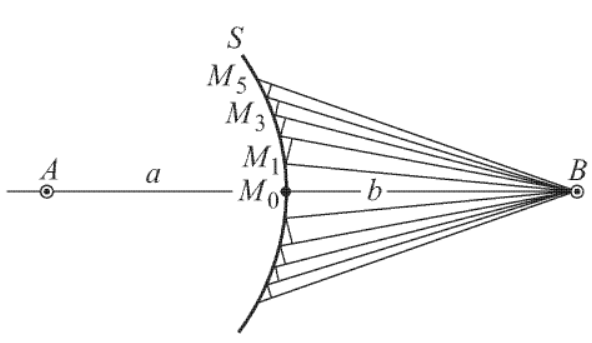
\includegraphics[width = 0.4\textwidth]{431-2.png}
		\end{center}
		\caption{Построение зон Френеля}
	\end{wrapfigure}
	Принцип Гюйгенса-Френеля:\\
	\textit{Каждый элемент волнового фронта можно рассматривать как центр  вторичного возмущения, порождающего вторичные сферические волны, а результирующее световое поле  в каждой точке пространства будет определяться интерференцией этих волн.}\\
	Теперь рассмотрим первое применение этого принципа, получившее название \textit{метод зон Френеля}
	

	Для этого рассмотрим действие световой волны действующей из точки $A$ в какой-то точке $B$.
	В этом случае можно, взяв точку $M_0$ в качестве центра (см. рис. 1), построить ряд концентрических сфер, радиусы которых начинаются с $b$ и увеличиваются каждый раз на половину длины волны $\frac{\lambda}{2}$. При пересечении с плоским фронтом волны $F$ эти сферы дадут концентрические окружности. Таким образом, на фронте волны появятся кольцевые зоны (зоны Френеля) с радиусами $r_1, r_2$ и т. д.
	
	Из геометрических соображений посчитав, можно получить, что 
	\begin{equation}
	r_i = i \sqrt{a \lambda}.
	\end{equation}
		\begin{wrapfigure}{r}{0.3\textwidth}
		\begin{center}
			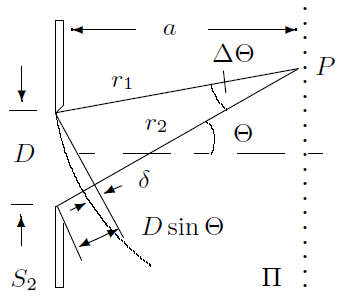
\includegraphics[width = 0.3\textwidth]{431-3.png}
		\end{center}
		\caption{К фазовым соотношениям при дифракции Фраунгофера}
	\end{wrapfigure}
	
	Картина дифракции упрощается, когда ширина щели становится значительно меньше ширины первой зоны Френеля, т.е. если 
	\begin{equation}
	D \ll\sqrt{a \lambda} 
	\end{equation}	
	Это условие всегда выполняется при достаточно большом $a$. В этом случае говорят, что \textit{дифракция Фраунгофера}. Дифракционную картину в этом случае называются \textit{дифракцией Фраунгофера}. При выполнении пункта $(2)$ у нас упрощаются фазовые соотношения, что поясняет рис. 2, в итоге с хорошим приближением можно считать, что разность хода между крайними лучами, приходящими от щели в точке наблюдения $P$, с хорошим приближением равна 
	\begin{equation}
	\Delta = r_2 - r_1 \approx D \sin \theta \approx D \cdot \theta
	\end{equation}
	Здесь предполагается, что $\theta$ достаточно мал.
	Дифракцию Фраунгофера можно наблюдать на установке рис. 1, но для удобства к подобной установке добавляется объектив $O_2$.
	
	\begin{figure}[h]
		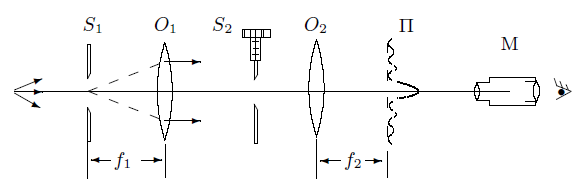
\includegraphics[width = 0.7\textwidth]{431-4.png}
		\centering
		\caption{Схема установки 2.}
	\end{figure}
	Дифракционная картина здесь наблюдается в фокальной плоскости объектива $O_2$. Каждому значению $\theta$ соответствует в этой плоскости точка, отстоящая от оптической оси на расстоянии 
	\begin{equation}
	X = f_2 \tan \theta \approx f_2 \theta.
	\end{equation}
	Объектив не вносит разности хода между интерферирующими лучам, поэтому в его фокальной плоскости наблюдается неискажённая дифракционная картина. При $\theta = 0$ разность хода между лучами нулевая, поэтому в центре поля зрения дифракционный максимум. Первый минимум соответствует $\theta_1$ такому, что в точке наблюдения разность хода пробегаем все значения от 0 до $2\pi$. Аналогично рассуждая, для $m$-й полосы
	\begin{equation}
	\theta_m = \frac{m \lambda}{D}
	\end{equation}
	Расстояние $X_m$ тёмной полосы от оптической оси из (5) и (6)
	\begin{equation}
	X_m = f_2m\frac{\lambda}{D}
	\end{equation}
	\subsection*{В. Дифракция Фраунгофера для двух щелей}
	Для наблюдения дифракции Фраунгофера на двух щелях $S_2$ заменим экраном Э с двумя щелями. При этом для оценки влияния ширины входной щели на чёткость вместо $S_1$ поставим щель с микрометрическим винтом.
	\begin{figure}[h]
		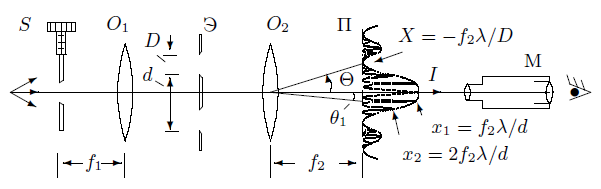
\includegraphics[width = 0.7\textwidth]{431-5.png}
		\centering
		\caption{Схема установки В.}
	\end{figure}
	Два дифракционных изображения входной щели, одно из которых образовано лучами, прошедшими через левую, а другое -- через правую щели, накладываются друг на друга.
	Если входная щель достаточно узка, то дифракционная картина в плоскости П подобна той, что получалась при дифракции на одной щели, однако вся картинка испещерена рядом дополнительных узких полос, наличие которых объясняется суперпозицией световых волн через разные щели. Светлая интерфереционная полоса наблюдается в случаях, когда разность хода равна целому числу длин волн. Таким образом, угловая координата максимума порядка $m$ равна
	\begin{equation}
	\theta_m = \dfrac{m \lambda}{d},
	\end{equation}
	где $d$ -- расстояние между щелями. Отсюда расстояние между соседними интерфереционными полосами в плоскости П равно
	\begin{equation}
	\delta x = f_2 \dfrac{\lambda}{d}
	\end{equation}
	Число интерференционных полос укладывающихся в области центрального максимума равна отношению ширины главного максимума $\frac{2\lambda f_2}{D}$ к расстоянию между соседними полосами:
	\begin{equation}
	n = \dfrac{2\lambda f_2}{D} \dfrac{1}{\delta f}= \dfrac{2d}{D}.
	\end{equation}
	При дифракции света на двух щелях чёткая система интерференционных полос наблюдается только при достаточно узкой ширине входной щели $S$. При увеличении ширины картинка пропадает и появляется вновь, но полосы при этом сильно размыты и видны плохо.
	\subsection*{Г. Влияние дифракции на разрешающую способность оптического инструмента}
	\begin{figure}[h]
		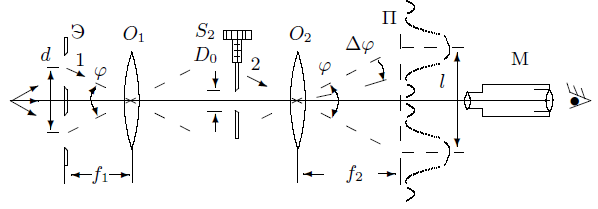
\includegraphics[width = 0.8\textwidth]{431-6.png}
		\centering
		\caption{Схема установки 4.}
	\end{figure}
	В отсутствие щели $S_2$ линзы $O_1$ и $O_2$ создают на плоскости П изоюражение щели $S_1$ и это изображение рассматриваются микроскопом М. Таким образом, установку можно рассматривать как оптический инструмент, предназначенные для получения изображения предмета. Если перед $O_2$ расположить $S_2$, то изображение объекта будет искажено из-за дифракции. Чем меньше ширина щели, тем сильнее искажение. Качественной характеристикой этого искажения может служить $\varphi_{min}$ --- минимальное угловое расстояние между объектами (источниками), которые всё ещё воспринимаются как раздельные. Поместим вместо $S_1$ экран Э с двумя щелями с расстоянием $d$. Тогда на $S_2$ будут падать два пучка света с углом
	\begin{equation}
	\varphi = \dfrac{d}{f_1}
	\end{equation}
	Из геометрии расстояние $l$ между изображениями щелей в плоскости П равно 
	\begin{equation}
	l = \varphi f_2 = d \dfrac{f_2}{f_1}.
	\end{equation}
	Ширина $\Delta \varphi$ определяется дифракцией на $S_2$. Условия, при которых изображения различимы разные для разных наблюдателей, поэтому используют \textit{критерий Рэлея} -- \textit{максимум одного дифракционного пятна должен совпадать с минимумом другого}. В наших условиях это значит, что угловая полуширина $\frac{\lambda}{D}$ равна угловому расстоянию $\frac{l}{f_2}$.
	
\section*{Ход работы}
\subsection*{А. Дифракция Френеля}
\begin{enumerate}
	\item Добившись наибольшей чёткости дифракционной картины, нашли резкое изображение щели (чёткие края без дифракционных полос). Начальное положение микроскопа --- координата по шкале линейки $x_0=343$ мм, расположенной на оптической скамье. 
	\item Приближая микроскоп к щели, сняли зависимость координаты микроскопа от числа $n$ наблюдаемых тёмных полос. Отметим, что эта серия измерений имеет довольно низкую точность из-за отклонений величины $x$, сравнимых с погрешностью.
	\begin{center}
		\begin{tabular}{|c|c|c|c|l|c|}
			\hline
			$n$, полос & 1 & 2 & 3 & 4 & 5 \\ \hline
			$x_n$, мм & 370 & 361 & 357 & 353 & 351 \\ \hline
		\end{tabular}
	\end{center}

Из формулы (1) найдём величину $2z_n$ и рассмотрим зависимость $2z_n(n)$, где длина волны зелёной линии ртути $\lambda = 546{,}1$ нм.
\begin{center}
	\begin{tabular}{|c|c|c|c|l|c|}
		\hline
		$n$, полос & 1 & 2 & 3 & 4 & 5 \\ \hline
		$2z_n$, мкм & $240\pm50$ & $280\pm20$ & $300\pm20$ & $290\pm15$ & $300\pm12$ \\ \hline
	\end{tabular}
\end{center}
Усреднённое значение размера зоны Френеля $<2z_n>=280\pm20$ мкм.
\item В соответствии с показаниями микрометрического винта ширина щели в данном опыте $D = 0{,}280\pm0{,}005$ мм. Измерения $D$, проведённые с помощью шкалы микроскопа, дают соответствующий результат: 
\begin{equation*}
D = 27\text{ дел.}\cdot 0{,}01 \text{ дел./мм} = 0{,}27\pm0{,}01\text{ мм}.
\end{equation*}
Получили, что размер зон Френеля примерно совпадает с шириной щели.

\item Вновь сфокусировали микроскоп на щель. При небольшом удалении микроскопа от щели у её краёв появляются узкие частые полосы. Это дифракция на краю экрана. Возле границы щели расположена самая яркая светлая полоса.
\item Для исследования дифракции Френеля на препятствии поставили вместо щели~$S_2$ рамку с тонкой вертикальной нитью. Настроили микроскоп на резкое изображение нити. При удалении микроскопа от нити на её фоне всегда наблюдается чётное число тёмных дифракционных полос (светлый центр).
\end{enumerate}
\subsection*{Б. Дифракция Фраунгофера на щели}
\begin{enumerate}
	\item Фокусное расстояние линз $f_{O_1} = 10{,}0$ см, $f_{O_2} = 16{,}0$ см. Диаметр щели по показаниям микрометрического винта $D = 135\pm5$ мкм. Дифракционная картина очень слабо разрешима, получены координаты только первых двух минимумов. Измерения проводились по шкале с длиной деления~$0{,}04$~мм.
	\begin{center}
		\begin{tabular}{|c|c|c|c|l|c|}
			\hline
			$m$ & -2 & -1 & 0 & 1 & 2 \\ \hline
			$k$, дел. & $0{,}80\pm0{,}05$ & $1{,}75\pm0{,}05$ & $2{,}80\pm0{,}05$ & $4{,}25\pm0{,}05$ & $5{,}50\pm0{,}05$ \\ \hline
			\multicolumn{1}{|l|}{$x$, мкм} & \multicolumn{1}{l|}{$320\pm20$} & \multicolumn{1}{l|}{$700\pm20$} & \multicolumn{1}{l|}{$1120\pm20$} & $1700\pm20$ & \multicolumn{1}{l|}{$2200\pm20$} \\ \hline
		\end{tabular}
	\end{center}
	
\begin{figure}[!htb] \centering
	\begin{tikzpicture}
	\begin{axis}[
	width=15cm,
	height=8cm,
	xlabel={$m$},
	ylabel={$x$, мкм},
	grid=major
	]
	\addplot +[
	blue!20!black,
	mark = 0,
	only marks,
	] plot [
	error bars/.cd,
	x dir=both,
	y dir=both,
	y fixed = 2,
	x fixed = 0,
	] table [
	x = x,
	y = y
	] {431.dat};
	\addplot +[
	blue!20!black,
	mark = 0,
	] table [
	y={create col/linear regression={y=y}}]
	{431.dat};
	\end{axis}
	\end{tikzpicture}
	\caption{Координаты минимумов дифракции Фраунгофера}
\end{figure}

	\item По наклону графика методом наименьших квадратов определим среднее расстояние между соседними минимумами $\Delta X = 470\pm30$ мкм. Пользуясь этим результатом, с помощью формулы (7) получим значение $D$:
	\begin{equation*}
	D = \dfrac{f_2m\lambda}{X_m} = \dfrac{f_2 \lambda}{\Delta X} = 180\pm10\text{ мкм}.
	\end{equation*}
\end{enumerate}

\subsection*{В. Дифракция Фраунгофера для двух щелей}
\begin{enumerate}
	\item Получим на экране дифракционную картину и проведем измерения. Получим для 1 и 2 максимума слева и справа соответственно координаты:
\begin{center}
\begin{tabular}{|c|c|c|c|c|}
	\hline
	$m$ & -2 & -1 & 1 & 2 \\ \hline
	$d_m$, дел. & $0{,}95\pm0{,}05$ & $1{,}60\pm0{,}05$ & $1{,}50\pm0{,}05$ & $0{,}80\pm0{,}05$ \\ \hline
	$x_m$, мкм & $38\pm2$ & $80\pm2$ & $75\pm2$ & $32\pm2$ \\ \hline
\end{tabular}
\end{center}
	Число наблюдаемых полос для первых максимумов $n_1 = 7$, для вторых $n_2 = 3$.
	
	Тогда найдём $d$ по формуле (8):
	\begin{equation*}
	d = \dfrac{f_2\lambda}{\delta x} = 1{,}41\pm0{,}05\text{ мм}.
	\end{equation*}

\end{enumerate}
	\subsection*{Г. Влияние дифракции на разрешающую способность оптического инструмента}
\begin{enumerate}
	\item Изображения почти сливаются при значении $D_0 = 100 \pm5 \text{ мкм}$. Заметим, что для него выполняется критерий Релея (соотношение (12)) с учётом $\frac{\lambda}{D_0} = \frac{l}{f_2}$. При этом ширина щелей, измеренная микроскопом $D = 340$ мкм, а расстояние между щелями $d = 1{,}2$ мм.
\end{enumerate}

\section*{Вывод}

Изучили два основных типа дифракции: Френеля и Фраунгофера при разных размерах щели и провели качественные наблюдения этих явлений, а также экспериментально проверили справедливость теоретических формул.  

\end{document}
